% Asal-usul (tidak pernah dicetak): lihat sources/outline_sources.md (Tahun 1: struktur
% internal Bumi dari seismologi; model acuan; massa jenis, gravitasi dan tekanan di dalam
% Bumi; mineralogi mantel; litosfer dan astenosfer). Kurva dari figdata/bachelor-1/prem_profiles.py
% (data bersama data:prem) dan figdata/bachelor-1/refraction.py (kerak dua-lapisan generik); nilai
% soal latihan dan soal dihitung dalam kalkulator skrap Buku 3 calc/ch09.py.
\chapter{Bumi Berlapis}\label{ch:b1:layered-earth}

Pada 8 Oktober 1909 sebuah gempa mengguncang lembah Kupa, di tenggara Zagreb.
% ledger: skoko:mohorovicic
Andrija Mohorovičić, yang memimpin observatorium di sana, mengumpulkan seismogram yang terekam di seluruh Eropa dan memperhatikan sesuatu yang ganjil: hingga beberapa ratus kilometer dari episentrum, gelombang pertama datang dengan satu cara; lebih jauh, jenis gelombang pertama yang lain mengambil alih, seolah-olah sebagian energi telah menemukan jalan yang lebih cepat di kedalaman. Ia menjelaskannya dengan sebuah batas sekitar lima puluh kilometer di bawah permukaan, di bawah batas itu gelombang merambat lebih cepat: dasar \omterm{def:b1:layered-earth:layers}{kerak}. Seabad rekaman semacam itu, jutaan jumlahnya, telah mengubah batas pertama itu menjadi model acuan seluruh Bumi, lapis demi lapis, dengan kecepatannya, massa jenisnya, percepatan gravitasinya, dan tekanannya hingga ke pusat. Bab ini menunjukkan bagaimana sebuah batas ditemukan dari waktu tempuh, apa yang dikatakan model acuan, bagaimana profil massa jenis digambar dari kecepatan seismik saja lalu diperiksa terhadap massa dan momen inersia Bumi, \omterm{def:b1:rock-forming-minerals:mineral}{mineral} apa yang membentuk \omterm{def:b1:layered-earth:layers}{mantel} pada setiap kedalaman, apa yang menyusun inti, dan di mana cangkang kaku planet ini berakhir.

\begin{recall}
Gelombang P adalah gelombang kompresi, gelombang S adalah gelombang geser; gelombang S tidak merambat dalam cairan, dan bayangan P dan S dari inti memberikan jari-jari \omterm{def:b1:layered-earth:layers}{inti luar} yang cair (Buku 2, kelas 11). Gelombang dibiaskan pada suatu batas menurut hukum Snell, $\sin i_1/v_1 = \sin i_2/v_2$ (fisika). Dalam fluida diam tekanan bertambah dengan kedalaman sebagai $\mathrm dP = \rho g\,\mathrm dz$ (fisika, Sarjana Tahun ke-1). \omterm{def:b1:layered-earth:layers}{Kerak}, \omterm{def:b1:layered-earth:layers}{mantel}, dan inti diperkenalkan dalam Buku 1 (kelas 6).
\end{recall}

\section{Gelombang seismik dalam Bumi berlapis}

Kecepatan gelombang seismik bergantung pada modulus elastis batuan dan pada massa jenisnya. Buku-buku fisika menurunkannya dari persamaan elastisitas kontinum; di sini keduanya diambil sebagai diketahui.

\begin{proposition}[Kecepatan seismik]\label{prop:b1:layered-earth:speeds}
Dalam padatan elastis isotrop dengan massa jenis $\rho$, modulus bulk $K$ dan modulus geser $\mu$, gelombang P dan S merambat dengan laju
\[
  v_P = \sqrt{\frac{K + \tfrac43\mu}{\rho}}, \qquad v_S = \sqrt{\frac{\mu}{\rho}}.
\]
Dalam cairan $\mu = 0$: $v_S = 0$ dan tidak ada gelombang S yang merambat.
\end{proposition}
\admitted

Karena $K$ dan $\mu$ positif, $v_P > v_S$ selalu: di \omterm{def:b1:layered-earth:layers}{kerak} dan \omterm{def:b1:layered-earth:layers}{mantel} PREM, $v_P$ kira-kira $1.8$ hingga $1.9$ kali $v_S$, dan gelombang P tiba lebih dulu. Kedua kecepatan umumnya bertambah dengan kedalaman, karena tekanan mengeraskan batuan lebih daripada memampatkannya, sehingga sinar membelok kembali ke permukaan; dan pada beberapa kedalaman keduanya melompat.

\begin{definition}[Diskontinuitas seismik, Moho, batas inti--mantel dan batas inti dalam]
\label{def:b1:layered-earth:discontinuity}
Sebuah \emph{diskontinuitas seismik}\index{diskontinuitas seismik} adalah permukaan di dalam Bumi tempat kecepatan seismik, massa jenis, atau keduanya berubah secara tiba-tiba, dalam ketebalan yang kecil dibanding panjang gelombang seismik. \emph{Diskontinuitas Mohorovičić}\index{diskontinuitas Mohorovičić} (atau \emph{Moho}\index{Moho}) adalah dasar \omterm{def:b1:layered-earth:layers}{kerak}, tempat $v_P$ melompat hingga sekitar \qty{8}{km.s^{-1}}. \emph{Batas inti--mantel}\index{batas inti--mantel} adalah permukaan antara \omterm{def:b1:layered-earth:layers}{mantel} silikat padat dan \omterm{def:b1:layered-earth:layers}{inti luar} yang cair; \emph{batas inti dalam}\index{batas inti dalam} adalah permukaan antara \omterm{def:b1:layered-earth:layers}{inti luar} yang cair dan \omterm{def:b1:layered-earth:layers}{inti dalam} yang padat.
\end{definition}

\subsection{Pembiasan pada batas lapisan}

Ambil sebuah lapisan dengan tebal $h$ dan kecepatan $v_1$, yaitu \omterm{def:b1:layered-earth:layers}{kerak}, di atas ruang setengah dengan kecepatan $v_2 > v_1$, yaitu \omterm{def:b1:layered-earth:layers}{mantel}, serta sebuah sumber di permukaan. Tiga gelombang mencapai penerima pada jarak $x$. Gelombang langsung merambat dalam lapisan, dengan kecepatan $v_1$. Gelombang pantul memantul dari batas itu. Dan sinar yang menumbuk batas pada sudut kritis $i_c$, dengan $\sin i_c = v_1/v_2$, dibiaskan sepanjang batas, merambat di medium yang lebih cepat tepat di bawahnya dengan kecepatan $v_2$, dan mengirimkan energi kembali ke atas ke dalam lapisan pada sudut yang sama $i_c$ di sepanjang jalurnya.

\begin{definition}[Gelombang kepala, jarak persilangan]\label{def:b1:layered-earth:head-wave}
Sebuah \emph{gelombang kepala}\index{gelombang kepala} adalah gelombang yang merambat sepanjang suatu batas dengan kecepatan medium yang lebih cepat di bawahnya dan meninggalkannya ke atas pada sudut kritis. \emph{Jarak persilangan}\index{jarak persilangan} adalah jarak dari sumber, di luar mana gelombang kepala tiba lebih dulu daripada gelombang langsung.
\end{definition}

\begin{theorem}[Waktu tempuh pada Bumi dua-lapisan]\label{thm:b1:layered-earth:two-layer}
Di atas lapisan dengan tebal $h$ dan kecepatan $v_1$ yang bertumpu pada ruang setengah dengan kecepatan $v_2 > v_1$, sumber dan penerima di permukaan yang berjarak $x$ menghasilkan
\[
  t_{\text{langsung}} = \frac{x}{v_1}, \qquad
  t_{\text{kepala}} = \frac{x}{v_2} + \frac{2h\cos i_c}{v_1}
  \quad (x \ge 2h\tan i_c), \qquad \sin i_c = \frac{v_1}{v_2},
\]
dan \omterm{def:b1:layered-earth:head-wave}{gelombang kepala} tiba lebih dulu di luar \omterm{def:b1:layered-earth:head-wave}{jarak persilangan}
\[
  x_c = 2h\sqrt{\frac{v_2 + v_1}{v_2 - v_1}}.
\]
\end{theorem}

\begin{proof}
\omterm{def:b1:layered-earth:head-wave}{Gelombang kepala} turun pada sudut $i_c$ melalui lapisan, menempuh lintasan sepanjang $h/\cos i_c$, merambat di sepanjang batas sejauh $x - 2h\tan i_c$, lalu naik kembali sepanjang lintasan sepanjang $h/\cos i_c$. Waktu tempuhnya adalah
\[
  t_{\text{kepala}} = \frac{2h}{v_1\cos i_c} + \frac{x - 2h\tan i_c}{v_2}
  = \frac{x}{v_2} + \frac{2h}{v_1\cos i_c}\Bigl(1 - \frac{v_1\sin i_c}{v_2}\Bigr)
  = \frac{x}{v_2} + \frac{2h}{v_1\cos i_c}\,(1 - \sin^2 i_c),
\]
yaitu $x/v_2 + 2h\cos i_c/v_1$. Lintasan itu hanya ada jika jarak horizontalnya positif, $x \ge 2h\tan i_c$. Kedua waktu sama ketika $x(1/v_1 - 1/v_2) = 2h\cos i_c/v_1$; dengan $\cos i_c = \sqrt{v_2^2 - v_1^2}/v_2$,
\[
  x\,\frac{v_2 - v_1}{v_1 v_2} = \frac{2h\sqrt{(v_2 - v_1)(v_2 + v_1)}}{v_1 v_2},
\]
yang memberikan $x_c$. Di luar titik itu, garis \omterm{def:b1:layered-earth:head-wave}{gelombang kepala}, dengan gradien yang lebih kecil $1/v_2$, berada di bawah garis gelombang langsung.
\end{proof}

Pada grafik waktu tempuh terhadap jarak, gelombang langsung dan \omterm{def:b1:layered-earth:head-wave}{gelombang kepala} tampak sebagai dua garis lurus. Gradiennya adalah kebalikan kecepatan, $1/v_1$ dan $1/v_2$; garis \omterm{def:b1:layered-earth:head-wave}{gelombang kepala}, bila diperpanjang mundur hingga $x = 0$, memotong sumbu waktu di \emph{waktu intersep} $t_i = 2h\cos i_c/v_1$. Gelombang pantul, $t = \sqrt{x^2 + 4h^2}/v_1$, adalah hiperbola yang menyinggung garis \omterm{def:b1:layered-earth:head-wave}{gelombang kepala} di jarak kritis $2h\tan i_c$, tempat \omterm{def:b1:layered-earth:head-wave}{gelombang kepala} mulai terbentuk (\cref{exo:b1:layered-earth:10}).

\begin{omfigure}
\begin{tabular}{@{}c@{}}
\begin{tikzpicture}
\begin{axis}[width=0.86\linewidth, axis equal image, xmin=0, xmax=260, ymin=-62, ymax=8,
  axis x line=top, axis y line=left, axis line style={-}, clip=false,
  ylabel={kedalaman (km)}, ytick={-60,-35,0},
  yticklabels={60,35,0}, tick label style={font=\scriptsize}, label style={font=\small}]
\fill[brown!12] (axis cs:0,0) rectangle (axis cs:260,-35);
\fill[orange!18] (axis cs:0,-35) rectangle (axis cs:260,-62);
\draw[black!60] (axis cs:0,-35) -- (axis cs:260,-35);
\addplot[very thick, blue!70!black] table[x=x, y=z, unbounded coords=jump,
  restrict expr to domain={\coordindex}{0:1}] {figdata/out/bachelor-1-refraction-rays.dat};
\addplot[thick, dashed, green!45!black] table[x=x, y=z, unbounded coords=jump,
  restrict expr to domain={\coordindex}{3:5}] {figdata/out/bachelor-1-refraction-rays.dat};
\addplot[very thick, red!75!black] table[x=x, y=z, unbounded coords=jump,
  restrict expr to domain={\coordindex}{7:10}] {figdata/out/bachelor-1-refraction-rays.dat};
\node[font=\scriptsize, anchor=north west] at (axis cs:2,-36) {mantel, $v_2 = \qty{8.0}{km.s^{-1}}$};
\node[font=\scriptsize, anchor=center] at (axis cs:125,-17) {kerak, $v_1 = \qty{6.0}{km.s^{-1}}$, $h = \qty{35}{km}$};
\node[font=\scriptsize, red!75!black, anchor=north] at (axis cs:150,-36) {gelombang kepala sepanjang Moho};
\node[font=\scriptsize, green!45!black, anchor=south] at (axis cs:40,-20) {pantul};
\node[font=\scriptsize, blue!70!black, anchor=north] at (axis cs:125,-1) {langsung};
\fill (axis cs:0,0) circle (2pt);
\end{axis}
\end{tikzpicture}\\[2pt]
{\small (a) lintasan sinar (jarak dalam km)}\\[6pt]
\begin{tikzpicture}
\begin{axis}[omrecord, width=0.86\linewidth, height=6.0cm, xmin=0, xmax=400, ymin=0, ymax=70,
  xlabel={jarak $x$ (km)}, ylabel={waktu tempuh $t$ (s)}, tick label style={font=\scriptsize},
  label style={font=\small}, clip=false,
  legend style={font=\scriptsize, at={(0.03,0.97)}, anchor=north west, draw=none, fill=white, fill opacity=0.85}]
\addplot[very thick, blue!70!black] table[x=x, y=t_direct] {figdata/out/bachelor-1-refraction-times.dat};
\addlegendentry{langsung, gradien $1/v_1$}
\addplot[thick, dashed, green!45!black] table[x=x, y=t_reflected] {figdata/out/bachelor-1-refraction-times.dat};
\addlegendentry{pantul}
\addplot[very thick, red!75!black, unbounded coords=jump] table[x=x, y=t_head] {figdata/out/bachelor-1-refraction-times.dat};
\addlegendentry{gelombang kepala, gradien $1/v_2$}
\addplot[thin, dotted, red!75!black, domain=0:79.37] {x/8 + 7.717};
\draw[black!60, densely dashed] (axis cs:185.2,0) -- (axis cs:185.2,30.87);
\node[font=\scriptsize, anchor=north west] at (axis cs:187,8) {$x_c = \qty{185}{km}$};
\node[font=\scriptsize, anchor=east, red!75!black] at (axis cs:-3,7.7) {$t_i$};
\end{axis}
\end{tikzpicture}\\[2pt]
{\small (b) waktu tempuh}
\end{tabular}

\par\smallskip{\small Refraksi melalui \omterm{def:b1:layered-earth:layers}{kerak} setebal \qty{35}{km}, dengan \qty{6.0}{km.s^{-1}}, di atas \omterm{def:b1:layered-earth:layers}{mantel} dengan \qty{8.0}{km.s^{-1}} ((a) dalam skala sebenarnya). (a) Gelombang langsung merambat di sepanjang permukaan; gelombang pantul yang digambar adalah yang menumbuk \omterm{def:b1:layered-earth:discontinuity}{Moho} pada sudut kritis, \ang{48.6}; \omterm{def:b1:layered-earth:head-wave}{gelombang kepala} merambat di sepanjang \omterm{def:b1:layered-earth:discontinuity}{Moho} dan kembali pada sudut itu. (b) Waktu tiba: \omterm{def:b1:layered-earth:head-wave}{gelombang kepala} muncul pada jarak kritis, \qty{79}{km}, menyinggung pantulan, dan menyusul gelombang langsung pada \omterm{def:b1:layered-earth:head-wave}{jarak persilangan}, \qty{185}{km}. Perpanjangan titik-titik memberikan waktu intersep $t_i = \qty{7.7}{s}$.}
\end{omfigure}

\begin{method}[Kedalaman suatu batas dari profil refraksi]\label{met:b1:layered-earth:moho}
\begin{enumerate}
  \item Gambarkan waktu kedatangan pertama terhadap jarak, dan cocokkan satu garis lurus pada kedatangan dekat sumber serta satu garis lain pada kedatangan yang jauh.
  \item Kebalikan gradien memberikan $v_1$ dan $v_2$; lalu $\sin i_c = v_1/v_2$.
  \item Baca waktu intersep $t_i$ dari garis yang jauh pada $x = 0$, dan hitung $h = t_i v_1/(2\cos i_c)$; periksa dengan \omterm{def:b1:layered-earth:head-wave}{jarak persilangan}, $h = \tfrac12 x_c\sqrt{(v_2 - v_1)/(v_2 + v_1)}$.
  \item Sebuah batas hanya ditemukan jika $v_2 > v_1$: lapisan yang lebih lambat di bawah lapisan yang lebih cepat tidak menghasilkan \omterm{def:b1:layered-earth:head-wave}{gelombang kepala} dan tetap tersembunyi.
\end{enumerate}
\end{method}

Dua jenis kedatangan pertama Mohorovičić tepat sama dengan dua garis ini: gelombang langsung di \omterm{def:b1:layered-earth:layers}{kerak} dekat sumber, dan \omterm{def:b1:layered-earth:head-wave}{gelombang kepala} sepanjang puncak \omterm{def:b1:layered-earth:layers}{mantel} yang lebih jauh. Perkiraannya untuk ketebalan \omterm{def:b1:layered-earth:layers}{kerak} di kawasan itu, \qty{54}{km}, telah dikonfirmasi dalam orde besarnya, tetapi kedalaman \omterm{def:b1:layered-earth:discontinuity}{Moho} bervariasi dari satu tempat ke tempat lain. Di bawah samudra \omterm{def:b1:layered-earth:layers}{kerak} hanya sekitar \qty{5}{km} tebalnya; di bawah benua rata-ratanya sekitar \qty{30}{km}, dan jauh lebih tebal di bawah pegunungan besar. Untuk model acuannya, PREM menempatkan \omterm{def:b1:layered-earth:discontinuity}{Moho} pada \qty{11}{km} di bawah permukaan laut di bawah samudra dan pada \qty{35}{km} di bawah benua.
% ledger: skoko:mohorovicic, usgs:crust-thickness, prem:moho-average

\begin{history}[Andrija Mohorovičić]
\begin{minipage}[t]{0.76\linewidth}\vspace{0pt}
% ledger: skoko:mohorovicic
Andrija Mohorovičić (1857--1936) datang ke seismologi dari meteorologi: seorang guru, lalu dari 1891 hingga 1921 direktur observatorium meteorologi Zagreb, dan ia menerbitkan kajian meteorologi terakhirnya pada 1901. Pada seismogram gempa lembah Kupa 8 Oktober 1909 ia menemukan dua pasang fase P dan S yang berbeda: dekat sumber, satu jenis gempa pertama tiba lebih dulu, dan lebih jauh, jenis lain, yang telah merambat lebih cepat di kedalaman. Pembacaannya atas kedua kedatangan ini sebagai gelombang langsung dan gelombang yang dibiaskan di bawah suatu batas menghasilkan batas yang kini menyandang namanya, serta pengukuran pertama ketebalan \omterm{def:b1:layered-earth:layers}{kerak}.
\end{minipage}\hfill
\begin{minipage}[t]{0.2\linewidth}\vspace{0pt}
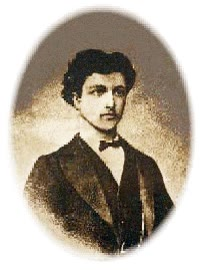
\includegraphics[width=\linewidth]{images/book3/b1-mohorovicic.jpg}

{\scriptsize Andrija Mohorovičić. Domain publik.}
\end{minipage}
\end{history}

\section{Model acuan Bumi}

Penalaran yang sama, diterapkan pada jutaan waktu tempuh di semua jarak dan pada periode osilasi bebas Bumi (seluruh planet berdering seperti lonceng sesudah gempa besar), menghasilkan kecepatan pada setiap kedalaman.

\begin{definition}[Model acuan Bumi]\label{def:b1:layered-earth:reference-model}
Sebuah \emph{model acuan Bumi}\index{model acuan Bumi} adalah Bumi yang simetris bola, diberikan sebagai kecepatan seismik $v_P(r)$ dan $v_S(r)$, massa jenis $\rho(r)$ dan, pada model yang paling lengkap, redaman, sebagai fungsi jari-jari $r$ saja, yang mencocokkan waktu tempuh teramati, periode osilasi bebas, massa Bumi, dan momen inersianya. Yang paling luas dipakai adalah PREM, model acuan Bumi preliminer (1981).
\end{definition}

PREM dicocokkan dengan jari-jari \qty{6371}{km}, massa \qty{5.974e24}{kg} dan \omterm{def:b1:comparative-planetology:moi}{faktor momen inersia} $0.3308$ Bumi. Ia membagi planet ini menjadi beberapa wilayah yang dihubungkan oleh diskontinuitas, dan profilnya (gambar di bawah) menunjukkan sekaligus lapisan-lapisan utamanya.

\begin{definition}[Kerak, mantel, inti luar, inti dalam]\label{def:b1:layered-earth:layers}
\emph{Kerak}\index{kerak} adalah lapisan silikat terluar di atas \omterm{def:b1:layered-earth:discontinuity}{Moho}. \emph{Mantel}\index{mantel} adalah cangkang silikat padat di antara \omterm{def:b1:layered-earth:discontinuity}{Moho} dan \omterm{def:b1:layered-earth:discontinuity}{batas inti--mantel}, pada kedalaman sekitar \qty{2891}{km}. \emph{Inti luar}\index{inti luar} adalah cangkang logam cair di antara \omterm{def:b1:layered-earth:discontinuity}{batas inti--mantel} dan \omterm{def:b1:layered-earth:discontinuity}{batas inti dalam}, pada kedalaman sekitar \qty{5150}{km}. \emph{Inti dalam}\index{inti dalam} adalah bola logam padat di bawahnya, dengan jari-jari sekitar \qty{1220}{km}.
\end{definition}

\begin{omfigure}
\begin{tikzpicture}
\begin{axis}[omrecord, omdepth, width=0.62\linewidth, height=5.4cm, xmin=0, xmax=14, ymin=0, ymax=6371,
  xlabel={kecepatan (\unit{km.s^{-1}}) atau massa jenis (\unit{g.cm^{-3}})}, ylabel={kedalaman (km)},
  ytick={0,1000,...,6000}, tick label style={font=\scriptsize}, label style={font=\small},
  clip=false, legend style={font=\scriptsize, at={(0.02,0.80)}, anchor=north west, draw=none, fill=white}]
\addplot[very thick, blue!70!black] table[x=vp, y=depth] {figdata/out/bachelor-1-prem_profiles-profiles.dat};
\addlegendentry{$v_P$}
\addplot[very thick, red!75!black] table[x=vs, y=depth] {figdata/out/bachelor-1-prem_profiles-profiles.dat};
\addlegendentry{$v_S$}
\addplot[very thick, black!70, densely dashed] table[x=rho, y=depth] {figdata/out/bachelor-1-prem_profiles-profiles.dat};
\addlegendentry{$\rho$}
\draw[black!35] (axis cs:0,670) -- (axis cs:14,670) node[right, font=\scriptsize, black] {670 km};
\draw[black!35] (axis cs:0,2891) -- (axis cs:14,2891) node[right, font=\scriptsize, black] {batas inti--mantel};
\draw[black!35] (axis cs:0,5149.5) -- (axis cs:14,5149.5) node[right, font=\scriptsize, black] {batas inti dalam};
\node[font=\scriptsize, anchor=west] at (axis cs:14,1700) {mantel};
\node[font=\scriptsize, anchor=west] at (axis cs:14,4000) {inti luar (cair)};
\node[font=\scriptsize, anchor=west] at (axis cs:14,5800) {inti dalam (padat)};
\end{axis}
\end{tikzpicture}

\par\smallskip{\small PREM: kecepatan gelombang P dan S serta massa jenis terhadap kedalaman. Kecepatan S turun menjadi nol di \omterm{def:b1:layered-earth:layers}{inti luar} yang cair dan muncul kembali, kecil, di \omterm{def:b1:layered-earth:layers}{inti dalam} yang padat; pada \omterm{def:b1:layered-earth:discontinuity}{batas inti--mantel} massa jenisnya hampir berlipat dua sementara $v_P$ turun dari 13.7 menjadi \qty{8.1}{km.s^{-1}}; lompatan dekat \qty{400}{km} dan \qty{670}{km} membatasi zona transisi.}
\end{omfigure}

\begin{table}[htbp]
\centering
\footnotesize
\setlength{\tabcolsep}{3pt}
\begin{tabular}{>{\raggedright\arraybackslash}p{0.2\linewidth}rr>{\raggedright\arraybackslash}p{0.47\linewidth}}
\hline
batas dalam PREM & kedalaman (km) & jari-jari (km) & apa yang berubah \\
\hline
\omterm{def:b1:layered-earth:discontinuity}{Moho} & 24.4 & 6346.6 & \omterm{def:b1:layered-earth:layers}{kerak} di atas, peridotit di bawah; $v_P$ 6.8 hingga 8.1 \\
diskontinuitas 220 km & 220 & 6151 & dasar \omterm{def:b1:layered-earth:lithosphere}{zona kecepatan rendah} dalam PREM \\
diskontinuitas 400 km & 400 & 5971 & \omterm{def:b1:rock-forming-minerals:groups}{olivin} menjadi wadsleyit (\qty{410}{km} dalam sebagian besar kajian) \\
diskontinuitas 670 km & 670 & 5701 & ringwoodit menjadi bridgmanit dan ferropericlase (\qty{660}{km} dalam sebagian besar kajian) \\
\omterm{def:b1:layered-earth:discontinuity}{batas inti--mantel} & 2891 & 3480 & silikat menjadi besi cair; $v_S$ 7.3 hingga 0; $\rho$ 5.57 hingga 9.90 \\
\omterm{def:b1:layered-earth:discontinuity}{batas inti dalam} & 5149.5 & 1221.5 & besi cair menjadi padat; $v_S$ 0 hingga 3.5; $\rho$ 12.17 hingga 12.76 \\
\hline
\end{tabular}
\caption{Diskontinuitas utama PREM (kecepatan dalam \unit{km.s^{-1}}, massa jenis dalam \unit{g.cm^{-3}}). PREM merata-ratakan \omterm{def:b1:layered-earth:layers}{kerak} menjadi \qty{24.4}{km}; \omterm{def:b1:layered-earth:layers}{kerak} nyata berkisar dari sekitar \qty{5}{km} di bawah samudra hingga beberapa puluh kilometer di bawah pegunungan.}
% ledger: usgs:crust-thickness
\label{tab:b1:layered-earth:prem}
\end{table}

Dua fakta dalam profil ini teramati secara langsung. Hilangnya $v_S$ di \omterm{def:b1:layered-earth:layers}{inti luar} adalah bayangan gelombang S yang disebutkan di atas: gelombang S masuk ke inti hanya sebagai gelombang P, karena inti tidak dapat meneruskan geseran, sehingga ia cair. Dan \omterm{def:b1:layered-earth:layers}{inti dalam} meneruskan gelombang S, pelan: ia padat. Fakta kedua itu berasal dari kedatangan P yang lemah di tempat gelombang P seharusnya tidak ada.

\begin{history}[Inge Lehmann dan inti dalam]
% ledger: hjortenberg:lehmann
\begin{minipage}[t]{0.76\linewidth}\vspace{0pt}
Inge Lehmann (1888--1993), kepala departemen seismologi lembaga geodesi Denmark, mempelajari rekaman gempa Buller 1929 di Selandia Baru dan menemukan gelombang P yang tiba di dalam zona bayangan, tempat inti seharusnya membelokkannya menjauh. Dalam sebuah makalah 1936 dengan judul terpendek, \emph{P$'$}, ia menunjukkan bahwa gelombang itu dapat dijelaskan jika inti memuat \omterm{def:b1:layered-earth:layers}{inti dalam} yang lebih kecil dengan kecepatan P yang lebih tinggi, yang mengembalikan sebagian energi ke arah permukaan. \omterm{def:b1:layered-earth:layers}{Inti dalamnya} kini diketahui padat, dan tumbuh perlahan seiring Bumi mendingin. Ia juga menemukan diskontinuitas dekat \qty{220}{km} yang menyandang namanya.
\end{minipage}\hfill
\begin{minipage}[t]{0.2\linewidth}\vspace{0pt}
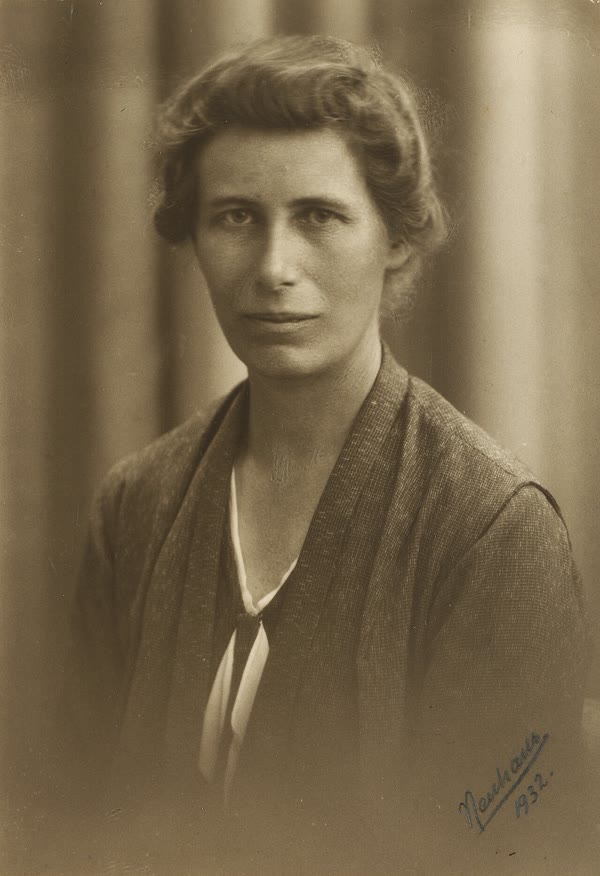
\includegraphics[width=\linewidth]{images/book3/b1-lehmann.jpg}

{\scriptsize Inge Lehmann pada 1932, oleh Even Neuhaus. Domain publik.}
\end{minipage}
\end{history}

\section{Massa jenis, gravitasi dan tekanan dari data seismik}

Kecepatan seismik memberi dua kombinasi modulus dan massa jenis, bukan massa jenis itu sendiri. Relasi ketiga berasal dari anggapan bahwa, di dalam lapisan dengan komposisi seragam, batuan hanya termampatkan oleh berat batuan di atasnya.

\begin{definition}[Parameter seismik]\label{def:b1:layered-earth:seismic-parameter}
\emph{Parameter seismik}\index{parameter seismik} pada suatu kedalaman adalah
\[
  \Phi = v_P^2 - \tfrac43 v_S^2 = \frac{K}{\rho},
\]
modulus bulk dibagi massa jenis, dihitung dari dua kecepatan seismik saja (\cref{prop:b1:layered-earth:speeds}).
\end{definition}

\begin{theorem}[Persamaan Adams--Williamson]\label{thm:b1:layered-earth:adams-williamson}
Dalam suatu wilayah dengan komposisi seragam, dalam kesetimbangan hidrostatik, termampatkan secara adiabatik, massa jenis bervariasi terhadap jari-jari sebagai
\[
  \frac{\mathrm d\rho}{\mathrm dr} = -\frac{\rho(r)\,g(r)}{\Phi(r)},
\]
dengan $g(r)$ adalah gravitasi pada jari-jari $r$.
\end{theorem}

\begin{proof}
Kesetimbangan hidrostatik memberikan $\mathrm dP/\mathrm dr = -\rho g$ (rekap di atas, dengan $\mathrm dz = -\mathrm dr$). Modulus bulk didefinisikan oleh $K = \rho\,\mathrm dP/\mathrm d\rho$ untuk pemampatan yang dibahas; untuk batuan dengan komposisi tetap yang termampatkan tanpa pertukaran panas, itu adalah modulus adiabatik yang diukur gelombang seismik, sehingga $\mathrm d\rho/\mathrm dP = \rho/K$. Dengan aturan rantai,
\[
  \frac{\mathrm d\rho}{\mathrm dr} = \frac{\mathrm d\rho}{\mathrm dP}\,
  \frac{\mathrm dP}{\mathrm dr} = \frac{\rho}{K}\,(-\rho g) = -\frac{\rho g}{K/\rho}
  = -\frac{\rho g}{\Phi}. \qedhere
\]
\end{proof}

Persamaan ini gagal pada suatu diskontinuitas, tempat komposisi atau struktur kristal berubah, dan di mana pun suhu menyimpang dari adiabat; tetapi di antara diskontinuitas ia menjelaskan dengan sangat baik peningkatan massa jenis yang teramati terhadap kedalaman (panel (c) gambar di bawah). Dengan memulai dari massa jenis di puncak setiap wilayah, mengintegralkannya ke bawah, dan menyesuaikan nilai awal hingga massa dan momen inersia tepat, begitulah model massa jenis pertama dibangun. Kedua bilangan global itu adalah integral massa jenis.

\begin{proposition}[Massa, gravitasi, tekanan dan momen inersia]
\label{prop:b1:layered-earth:integrals}
Untuk Bumi simetris bola dengan jari-jari $R$ dan massa jenis $\rho(r)$, massa di dalam jari-jari $r$, gravitasi, tekanan, dan momen inersia terhadap sumbu yang melalui pusat adalah
\[
  m(r) = \int_0^r 4\pi s^2\rho(s)\,\mathrm ds, \quad
  g(r) = \frac{G\,m(r)}{r^2}, \quad
  P(r) = \int_r^R \rho(s)\,g(s)\,\mathrm ds, \quad
  I = \frac{8\pi}{3}\int_0^R \rho(r)\,r^4\,\mathrm dr.
\]
\end{proposition}

\begin{proof}
Kulit tipis dengan jari-jari $s$ dan tebal $\mathrm ds$ memiliki volume $4\pi s^2\,\mathrm ds$, maka diperoleh integral pertama. Gravitasi suatu benda simetris bola di luar suatu jari-jari sama dengan gravitasi massa di dalamnya, terpusat di pusat, dan kulit-kulit di luar $r$ menarik dengan gaya bersih nol (teorema kulit, diterima dari buku-buku fisika); maka diperoleh $g(r)$. Dengan mengintegralkan persamaan hidrostatik dari permukaan, tempat $P = 0$, diperoleh $P(r)$. Untuk momen inersia, sebuah kulit bola tipis dengan massa $\mathrm dm$ dan jari-jari $r$ memiliki, terhadap ketiga sumbu $x$, $y$, $z$, momen yang jumlahnya adalah
$\int (y^2 + z^2) + (z^2 + x^2) + (x^2 + y^2)\,\mathrm dm = 2r^2\,\mathrm dm$;
Menurut simetri, ketiganya sama, sehingga masing-masing adalah $\tfrac23 r^2\,\mathrm dm$. Dengan $\mathrm dm = 4\pi r^2\rho\,\mathrm dr$, penjumlahan kulit-kulit memberikan $I$.
\end{proof}

Untuk bola dengan massa jenis seragam, $I = \tfrac{8\pi}{15}\rho R^5 = 0.4\,MR^2$.
Faktor Bumi $I/MR^2 = 0.3308$ lebih kecil: massanya terkonsentrasi ke arah pusat, dan itu adalah argumen pertama untuk inti yang padat. Dihitung dari massa jenis PREM saja, integral-integral itu memberikan massa \qty{5.976e24}{kg} (\qty{0.06}{\percent} di atas \qty{5.972e24}{kg} yang terukur), faktor $0.3309$, dan tekanan pusat sebesar \qty{364}{GPa}, nilai yang ditabelkan bersama PREM hingga \qty{0.1}{\percent}.

\begin{omfigure}
\begin{tabular}{@{}c@{\hspace{2mm}}c@{\hspace{2mm}}c@{}}
\begin{tikzpicture}
\begin{axis}[omrecord, omdepth, width=0.35\linewidth, height=7.0cm, xmin=0, xmax=12, ymin=0, ymax=6371,
  xlabel={$g$ (\unit{m.s^{-2}})}, ylabel={kedalaman (km)}, ytick={0,1000,...,6000}, xtick={0,4,8,12},
  tick label style={font=\scriptsize}, label style={font=\small}]
\addplot[very thick, blue!70!black] table[x=g, y=depth] {figdata/out/bachelor-1-prem_profiles-functionals.dat};
\draw[black!35] (axis cs:0,2891) -- (axis cs:12,2891);
\draw[black!35] (axis cs:0,5149.5) -- (axis cs:12,5149.5);
\node[font=\scriptsize, anchor=south west] at (axis cs:0.3,2891) {CMB};
\node[font=\scriptsize, anchor=south west] at (axis cs:0.3,5149.5) {ICB};
\end{axis}
\end{tikzpicture}
&
\begin{tikzpicture}
\begin{axis}[omrecord, omdepth, width=0.35\linewidth, height=7.0cm, xmin=0, xmax=400, ymin=0, ymax=6371,
  xlabel={$P$ (GPa)}, ytick={0,1000,...,6000}, yticklabels={}, xtick={0,200,400},
  tick label style={font=\scriptsize}, label style={font=\small}]
\addplot[very thick, red!75!black] table[x=P, y=depth] {figdata/out/bachelor-1-prem_profiles-functionals.dat};
\draw[black!35] (axis cs:0,2891) -- (axis cs:400,2891);
\draw[black!35] (axis cs:0,5149.5) -- (axis cs:400,5149.5);
\node[font=\scriptsize, anchor=south west] at (axis cs:150,2891) {\qty{136}{GPa}};
\node[font=\scriptsize, anchor=south east] at (axis cs:290,5149.5) {\qty{329}{GPa}};
\end{axis}
\end{tikzpicture}
&
\begin{tikzpicture}
\begin{axis}[omrecord, omdepth, width=0.35\linewidth, height=7.0cm, xmin=2, xmax=14, ymin=0, ymax=6371,
  xlabel={$\rho$ (\unit{g.cm^{-3}})}, ytick={0,1000,...,6000}, yticklabels={}, xtick={2,6,10,14},
  tick label style={font=\scriptsize}, label style={font=\small},
  legend style={font=\scriptsize, at={(0.97,0.97)}, anchor=north east, draw=none, fill=white}]
\addplot[very thick, black!55] table[x=rho, y=depth] {figdata/out/bachelor-1-prem_profiles-profiles.dat};
\addlegendentry{PREM}
\addplot[only marks, mark=o, mark size=1.4pt, orange!85!black, each nth point=15, unbounded coords=discard]
  table[x=rho_aw, y=depth] {figdata/out/bachelor-1-prem_profiles-adams.dat};
\addlegendentry{Adams--Williamson}
\end{axis}
\end{tikzpicture}
\\[2pt]
{\small (a) gravitasi} & {\small (b) tekanan} & {\small (c) pemampatan diri}
\end{tabular}

\par\smallskip{\small Di dalam Bumi, dari PREM. (a) dan (b) Gravitasi dan tekanan dihitung dari massa jenis PREM dengan \cref{prop:b1:layered-earth:integrals}: gravitasi tetap dekat \qty{10}{m.s^{-2}} sepanjang \omterm{def:b1:layered-earth:layers}{mantel}, mencapai puncak \qty{10.7}{m.s^{-2}} di \omterm{def:b1:layered-earth:discontinuity}{batas inti--mantel} (CMB) dan turun menjadi nol di pusat; tekanan mencapai \qty{136}{GPa} di CMB, \qty{329}{GPa} di \omterm{def:b1:layered-earth:discontinuity}{batas inti dalam} (ICB), dan \qty{364}{GPa} di pusat. (c) Persamaan Adams--Williamson, diintegralkan ke bawah dari massa jenis PREM pada \qty{771}{km} dan dari puncak \omterm{def:b1:layered-earth:layers}{inti luar} dengan kecepatan dan gravitasi PREM (lingkaran), mengikuti PREM hingga dalam \qty{0.2}{\percent}: di sana kenaikan massa jenis adalah pemampatan bahan yang seragam; lompatan-lompatannya tidak.}
\end{omfigure}

Bahwa gravitasi bertambah dalam perjalanan ke bawah melalui \omterm{def:b1:layered-earth:layers}{mantel} adalah akibat langsung dari inti yang padat: massa yang tersisa di dalam jari-jari menurun lebih lambat daripada $r^2$. Melalui \omterm{def:b1:layered-earth:layers}{mantel} $g$ hampir tidak berubah, dan tekanan bertambah hampir linear terhadap kedalaman, sekitar \qty{4.7}{GPa} per seratus kilometer.


\section{Mantel: satu batuan, beberapa asosiasi mineral}

\omterm{def:b1:layered-earth:layers}{Mantel} atas adalah peridotit, dikenal dari fragmen yang dibawa gunung api ke permukaan dan dari irisan \omterm{def:b1:layered-earth:layers}{mantel} yang terdorong ke atas benua: sekitar separuh hingga tiga per lima \omterm{def:b1:rock-forming-minerals:groups}{olivin} menurut volume (\qtyrange{49}{62}{\percent} dalam komposisi yang diusulkan), sisanya \omterm{def:b1:rock-forming-minerals:groups}{piroksen} dan \omterm{def:b1:rock-forming-minerals:mineral}{mineral} beralumina (\omterm{def:b1:rock-forming-minerals:groups}{plagioklas}, spinel atau \omterm{def:b1:rock-forming-minerals:groups}{garnet}, bergantung pada kedalaman). Tekanan yang bertambah dengan kedalaman tidak mengubah komposisi ini, tetapi memaksa atomnya ke dalam susunan yang lebih padat: \omterm{def:b1:rock-forming-minerals:polymorph}{polimorf} (\cref{ch:b1:rock-forming-minerals}) muncul satu demi satu.

\begin{definition}[Zona transisi mantel]\label{def:b1:layered-earth:transition-zone}
\emph{Zona transisi mantel}\index{zona transisi mantel} adalah bagian \omterm{def:b1:layered-earth:layers}{mantel} di antara \omterm{def:b1:layered-earth:discontinuity}{diskontinuitas seismik} dekat kedalaman \qty{410}{km} dan \qty{660}{km}, tempat \omterm{def:b1:rock-forming-minerals:groups}{olivin} \omterm{def:b1:layered-earth:layers}{mantel} atas digantikan oleh \omterm{def:b1:rock-forming-minerals:polymorph}{polimorf-polimorfnya} yang lebih padat, wadsleyit lalu ringwoodit. Di atasnya terdapat \omterm{def:b1:layered-earth:layers}{mantel} atas; di bawahnya \omterm{def:b1:layered-earth:layers}{mantel} bawah, hingga \omterm{def:b1:layered-earth:discontinuity}{batas inti--mantel}.
\end{definition}

Pada sekitar \qty{410}{km} (\qty{14}{GPa}) \omterm{def:b1:rock-forming-minerals:groups}{olivin} \ce{(Mg,Fe)2SiO4} berubah menjadi wadsleyit, dengan rumus yang sama; dekat \qty{520}{km} (\qty{17.5}{GPa}) wadsleyit berubah menjadi ringwoodit; \omterm{def:b1:rock-forming-minerals:groups}{piroksen} larut ke dalam \omterm{def:b1:rock-forming-minerals:groups}{garnet} kaya silikon, majorit, hingga pada pertengahan zona transisi \omterm{def:b1:rock-forming-minerals:groups}{garnet} memuat semuanya, sehingga zona itu sedikit lebih dari separuh \omterm{def:b1:rock-forming-minerals:polymorph}{polimorf} \omterm{def:b1:rock-forming-minerals:groups}{olivin} dan sisanya \omterm{def:b1:rock-forming-minerals:groups}{garnet}. Pada sekitar \qty{660}{km}, pada tekanan dekat \qty{24}{GPa}, ringwoodit terurai menjadi dua \omterm{def:b1:rock-forming-minerals:mineral}{mineral}, ditulis untuk \omterm{def:b1:rock-forming-minerals:solid-solution}{anggota ujung} kaya magnesium
\[
  \ce{Mg2SiO4 -> MgSiO3 + MgO}:
\]
bridgmanit, \ce{(Mg,Fe)SiO3} dengan struktur perovskit, dan ferropericlase, \ce{(Mg,Fe)O}. \omterm{def:b1:layered-earth:layers}{Mantel} bawah dengan komposisi yang sama seperti \omterm{def:b1:layered-earth:layers}{mantel} atas kira-kira \qty{75}{\percent} bridgmanit, \qty{17}{\percent} ferropericlase dan \qty{8}{\percent} perovskit silikat kalsium menurut volume, dan cocok dengan massa jenis serta kecepatan model acuan. Bridgmanit karena itu adalah \omterm{def:b1:rock-forming-minerals:mineral}{mineral} paling melimpah di Bumi; namanya baru diberikan pada 2014, setelah butir alami dideskripsikan dalam meteorit yang mengalami kejutan tekanan hebat.
% ledger: frost:mantle-transitions, sun:lower-mantle, tschauner:bridgmanite

Setiap perubahan menghasilkan \omterm{def:b1:rock-forming-minerals:mineral}{mineral} yang lebih padat, sehingga menaikkan massa jenis dan kecepatan seismik: transisi-transisi itu adalah diskontinuitas pada profil (gambar di bawah). Kedalamannya tidak tetap. Perubahan fase terjadi pada tekanan yang bergantung pada suhu, dan gradien ketergantungan itu (gradien Clapeyron, yang dibahas dalam volume Sarjana Tahun ke-2) menggeser diskontinuitas \qty{410}{km} ke atas dan \qty{660}{km} ke bawah di batuan dingin lempeng yang tenggelam. Memetakan topografi diskontinuitas adalah salah satu cara menemukan wilayah dingin dan panas di \omterm{def:b1:layered-earth:layers}{mantel}.

\begin{omfigure}
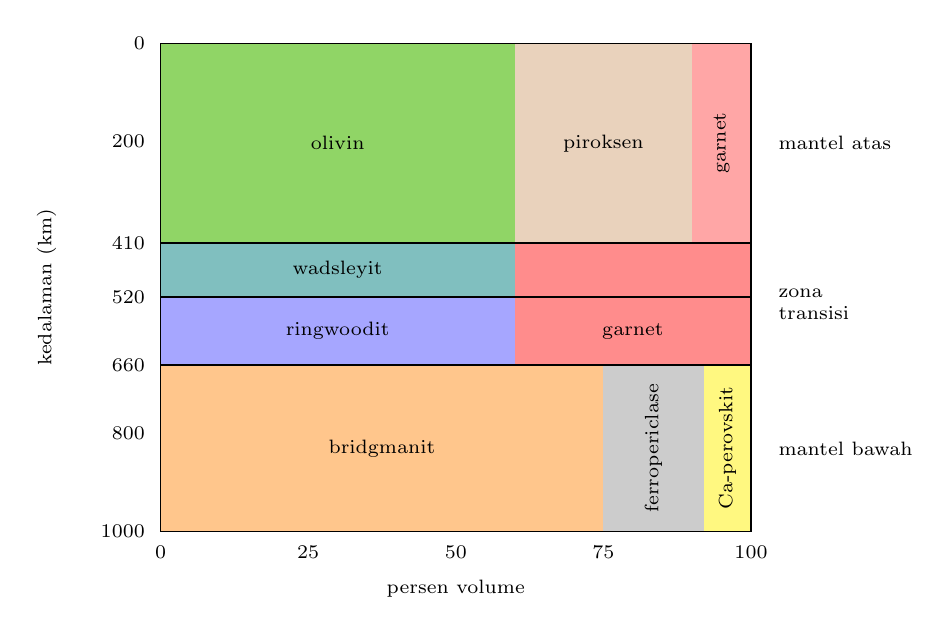
\begin{tikzpicture}[x=0.075mm, y=-0.062mm, font=\scriptsize]
% schematic volume fractions (ledger frost:mantle-transitions, sun:lower-mantle)
\def\W{1000}
% upper mantle 0-410: olivine 60, pyroxenes 30, garnet 10
\fill[green!45!olive!60] (0,0) rectangle (600,410);
\fill[brown!35] (600,0) rectangle (900,410);
\fill[red!35] (900,0) rectangle (1000,410);
% 410-520 wadsleyite 60, garnet 40 ; 520-660 ringwoodite 60, garnet 40
\fill[teal!50] (0,410) rectangle (600,520);
\fill[blue!35] (0,520) rectangle (600,660);
\fill[red!45] (600,410) rectangle (1000,660);
% 660-1000 bridgmanite 75, ferropericlase 17, Ca-perovskite 8
\fill[orange!45] (0,660) rectangle (750,1000);
\fill[gray!40] (750,660) rectangle (920,1000);
\fill[yellow!50] (920,660) rectangle (1000,1000);
\draw (0,0) rectangle (1000,1000);
\foreach \d in {410,520,660} \draw[thick] (0,\d) -- (1000,\d);
\node at (300,205) {olivin};
\node[align=center] at (750,205) {piroksen};
\node[rotate=90] at (950,205) {garnet};
\node at (300,465) {wadsleyit};
\node at (300,590) {ringwoodit};
\node[align=center] at (800,590) {garnet};
\node at (375,830) {bridgmanit};
\node[rotate=90, align=center] at (835,830) {ferropericlase};
\node[rotate=90] at (960,830) {Ca-perovskit};
\foreach \d in {0,200,410,520,660,800,1000} \node[anchor=east] at (-10,\d) {\d};
\node[rotate=90, anchor=south] at (-160,500) {kedalaman (km)};
\foreach \p in {0,25,50,75,100} \node[anchor=north] at (\p*10,1010) {\p};
\node[anchor=north] at (500,1080) {persen volume};
\node[anchor=west, align=left] at (1030,205) {mantel atas};
\node[anchor=west, align=left] at (1030,535) {zona\\transisi};
\node[anchor=west, align=left] at (1030,830) {mantel bawah};
\end{tikzpicture}

\par\smallskip{\small \omterm{def:b1:rock-forming-minerals:mineral}{Mineral-mineral} peridotit \omterm{def:b1:layered-earth:layers}{mantel} terhadap kedalaman, sebagai fraksi volume (skematis: batasnya digambar tajam, dan fraksinya nilai bulat dalam rentang yang dikutip dalam teks). Komposisinya tidak berubah; \omterm{def:b1:rock-forming-minerals:mineral}{mineralnya} berubah, pada sekitar 410, 520 dan \qty{660}{km}.}
\end{omfigure}

Di dasar \omterm{def:b1:layered-earth:layers}{mantel}, lapisan yang disebut D$''$ (D dua-prima, nama yang dipertahankan dari model awal Bumi) memiliki gradien kecepatan yang berbeda dari bagian lain \omterm{def:b1:layered-earth:layers}{mantel} bawah; PREM memberinya \qty{150}{km} terbawah \omterm{def:b1:layered-earth:layers}{mantel}. Lapisan ini heterogen secara seismik: bercak-bercak kecepatan sangat rendah, gradien curam, reflektor. Diperkirakan ia adalah lapisan batas antara inti yang panas dan \omterm{def:b1:layered-earth:layers}{mantel}, dan mungkin kuburan lempeng-lempeng tua.
% ledger: prem:dpp

\section{Inti}

Inti sebagian besar terdiri atas besi. Massa jenisnya, kecepatannya, dan kemampuannya membangkitkan medan magnet semuanya menunjuk ke logam, dan di antara unsur-unsur yang cukup berat dan yang tampak umum pada meteorit serta Matahari, besi jauh paling melimpah. Nikel, yang melimpah dalam meteorit besi, menyertainya. Tetapi inti bukan besi--nikel murni.
\begin{itemize}
  \item Inti \qtyrange{5}{10}{\percent} lebih ringan daripada besi murni pada tekanan dan suhu yang sama: ia harus mengandung unsur-unsur ringan, di antaranya silikon, belerang, karbon, oksigen, dan hidrogen adalah kandidatnya.
  \item Massa jenis melompat sekitar \qty{4.5}{\percent} pada \omterm{def:b1:layered-earth:discontinuity}{batas inti dalam}, terlalu besar untuk pembekuan satu logam yang sama: \omterm{def:b1:layered-earth:layers}{inti dalam} juga mengandung unsur ringan, tetapi lebih sedikit, beberapa persen dibandingkan \qtyrange{5}{10}{\percent} di cairan.
\end{itemize}
% ledger: badro:core
Perbedaan ini punya konsekuensi. Seiring Bumi mendingin --- \omterm{def:b1:layered-earth:layers}{mantelnya} kira-kira \qty{100}{\degreeCelsius} per miliar tahun saat ini --- cairan inti membeku ke \omterm{def:b1:layered-earth:layers}{inti dalam}, yang tumbuh, dan
% ledger: bellini:cooling
pembekuan menyisakan sebagian besar unsur ringan di dalam cairan. Cairan ringan yang dilepaskan di dasar \omterm{def:b1:layered-earth:layers}{inti luar} naik, dan daya apung ini diduga membantu mengaduk \omterm{def:b1:layered-earth:layers}{inti luar} serta menggerakkan dinamo yang menghasilkan medan magnet Bumi.

\section{Lapisan mekanik: litosfer dan astenosfer}

Lapisan di atas didefinisikan oleh komposisi dan fase: \omterm{def:b1:layered-earth:layers}{kerak} dan \omterm{def:b1:layered-earth:layers}{mantel} adalah batuan yang berbeda, \omterm{def:b1:layered-earth:layers}{inti luar} dan \omterm{def:b1:layered-earth:layers}{inti dalam} adalah keadaan yang berbeda. Tektonik lempeng memerlukan pembagian lain, berdasarkan kekuatan, yang memotong pembagian pertama.

\begin{definition}[Litosfer, astenosfer, zona kecepatan rendah]
\label{def:b1:layered-earth:lithosphere}
Sebuah \emph{litosfer}\index{litosfer} adalah cangkang luar Bumi yang kaku, yaitu \omterm{def:b1:layered-earth:layers}{kerak} dan \omterm{def:b1:layered-earth:layers}{mantel} paling atas, yang berperilaku sebagai lapisan kuat dalam waktu geologi dan terbagi menjadi lempeng. \emph{Astenosfer}\index{astenosfer} adalah lapisan yang lebih lemah di \omterm{def:b1:layered-earth:layers}{mantel} atas di bawahnya, yang berdeformasi dengan aliran lambat dan membiarkan lempeng bergerak. \emph{Zona kecepatan rendah}\index{zona kecepatan rendah} adalah rentang kedalaman di bawah litosfer tempat kecepatan seismik, terutama kecepatan S, lebih rendah daripada tepat di atas dan di bawahnya.
\end{definition}

\omterm{def:b1:layered-earth:lithosphere}{Litosfer} bukan batuan melainkan suatu rentang suhu: peridotit \omterm{def:b1:layered-earth:layers}{mantel} kuat di tempat yang dingin dan merayap di tempat yang panas, dan dasarnya kira-kira berupa isoterm. Ia tipis di bawah punggungan, tempat \omterm{def:b1:layered-earth:layers}{mantel} panas naik, sekitar \qty{140}{km} tebalnya di bawah dasar samudra tertua, dan \qtyrange{40}{280}{km} tebalnya di bawah benua, paling tebal di bawah kraton tua; puncak \omterm{def:b1:layered-earth:lithosphere}{astenosfer} terletak sekitar \qtyrange{80}{200}{km}. Secara seismik, \omterm{def:b1:layered-earth:lithosphere}{astenosfer} tampak sebagai \omterm{def:b1:layered-earth:lithosphere}{zona kecepatan rendah}, dekat dengan kondisi peleburannya: dalam PREM kecepatan S berkurang sedikit dari \omterm{def:b1:layered-earth:discontinuity}{Moho} ke bawah hingga \qty{220}{km}, tempat ia melompat naik lagi. Bagaimana kekuatan bergantung pada suhu, dan mengapa, menjadi pokok bahasan \cref{ch:b1:stress-strain-rheology}.

\begin{inthefield}[Stasiun seismik]
\begin{minipage}[t]{0.55\linewidth}\vspace{0pt}
Data waktu tempuh yang menjadi dasar model acuan berasal dari stasiun permanen. Seismometer pita-lebar, yang merekam gerakan tanah dari seperseratus detik hingga beberapa jam periodenya, berdiri di atas tiang beton yang dibangun di atas batuan dasar yang terbuka dan diisolasi dari lantai ruang bawah tanah, di bawah penutup yang menjaga suhunya tetap stabil: perubahan sepersekian derajat, hembusan angin, atau truk yang lewat akan tampak pada rekaman. Pencatat data memberi cap waktu pada setiap sampel dengan waktu dari satelit, dan rekaman dialirkan ke pusat data yang membagikannya secara terbuka. Jaringan stasiun semacam itu menentukan lokasi dan waktu setiap gempa besar; waktu kedatangan yang dipilih dari rekaman mereka diinversi menjadi kecepatan pada setiap kedalaman.
\end{minipage}\hfill
\begin{minipage}[t]{0.42\linewidth}\vspace{0pt}
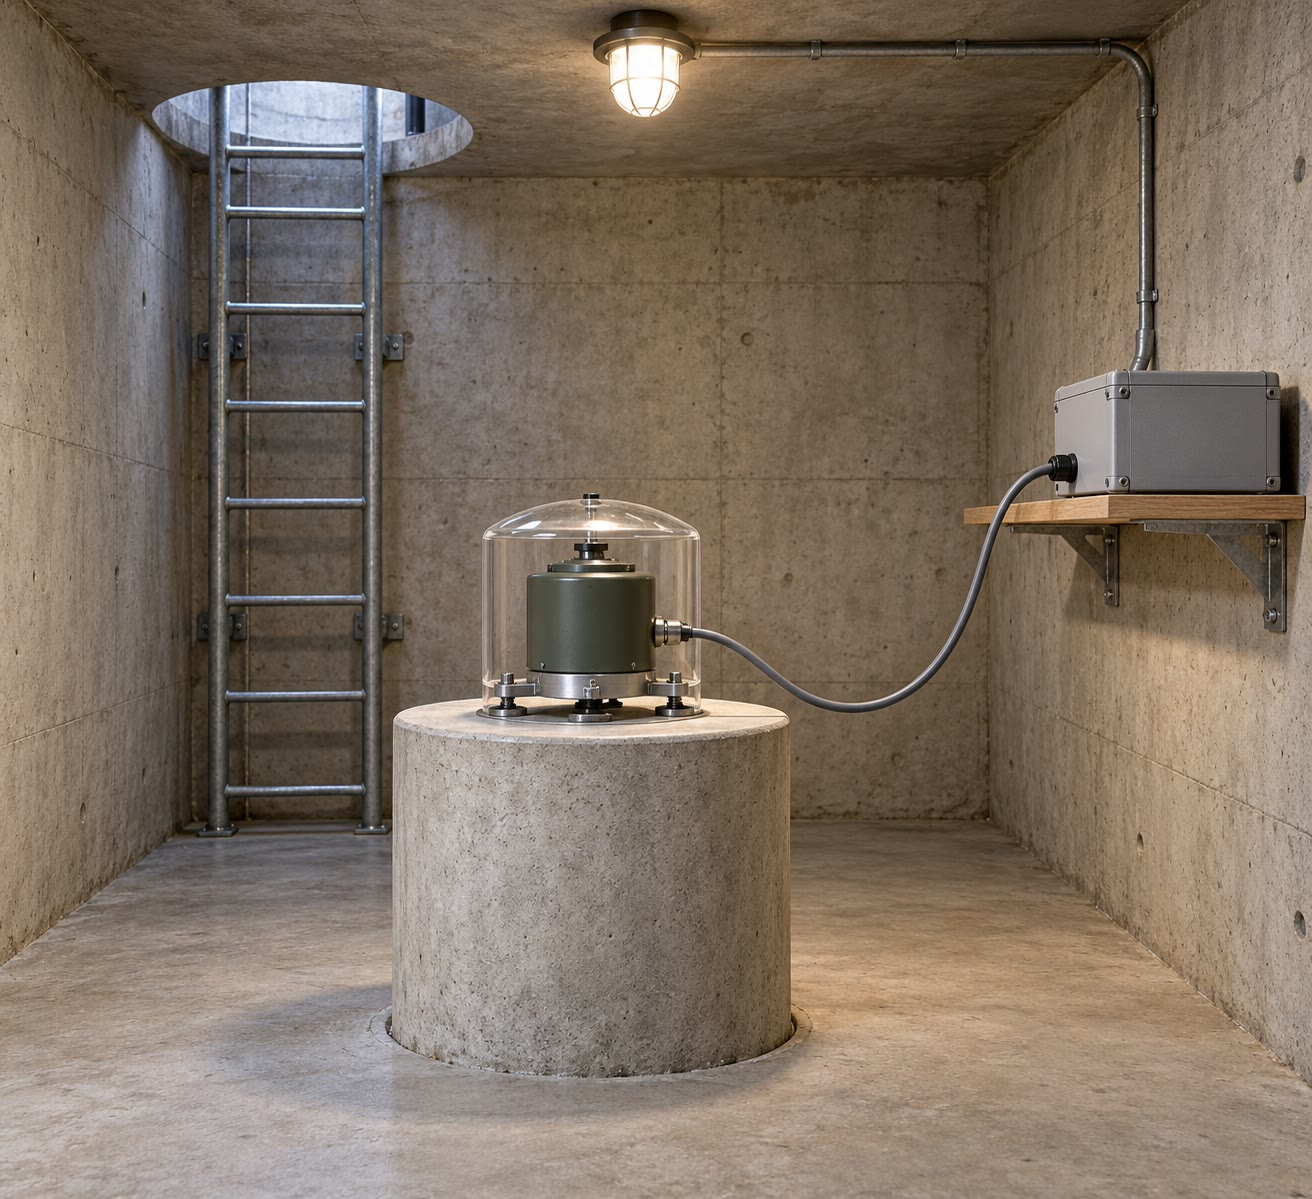
\includegraphics[width=\linewidth]{images/book3/ai/b1-seismometer-vault.jpg}

{\scriptsize Seismometer pita-lebar di atas tiangnya dalam ruang bawah tanah, dengan pencatat data di dinding (ilustrasi buatan AI).}
\end{minipage}
\end{inthefield}

\section{Latihan}

\begin{exercise}[$\star$]\label{exo:b1:layered-earth:1}
Dengan jari-jari PREM $R = \qty{6371}{km}$, $r_{\text{CMB}} = \qty{3480}{km}$ dan $r_{\text{ICB}} = \qty{1221.5}{km}$, hitung fraksi volume Bumi yang ditempati oleh inti dan oleh \omterm{def:b1:layered-earth:layers}{inti dalam}.
% ledger: prem:cmb, prem:icb
\end{exercise}

\begin{exercise}[$\star$]\label{exo:b1:layered-earth:2}
Tepat di atas \omterm{def:b1:layered-earth:discontinuity}{batas inti--mantel} PREM memberikan $v_P = \qty{13.7166}{km.s^{-1}}$, $v_S = \qty{7.26466}{km.s^{-1}}$, $\rho = \qty{5.56645}{g.cm^{-3}}$; tepat di bawahnya, $v_P = \qty{8.06482}{km.s^{-1}}$, $v_S = 0$, $\rho = \qty{9.90349}{g.cm^{-3}}$. Hitung \omterm{def:b1:layered-earth:seismic-parameter}{parameter seismik} dan modulus bulk di setiap sisi (dalam GPa). Apa yang berubah paling banyak di seberang batas?
% ledger: data:prem, prem:cmb
\end{exercise}

\begin{exercise}[$\star$]\label{exo:b1:layered-earth:3}
\omterm{def:b1:layered-earth:layers}{Kerak} setebal \qty{30}{km}, dengan kecepatan \qty{6.2}{km.s^{-1}}, bertumpu pada \omterm{def:b1:layered-earth:layers}{mantel} dengan \qty{8.1}{km.s^{-1}}. Hitung sudut kritis, jarak kritis, dan \omterm{def:b1:layered-earth:head-wave}{jarak persilangan}.
\end{exercise}

\begin{exercise}[$\star$]\label{exo:b1:layered-earth:4}
Massa inti adalah \qty{1.94e24}{kg} dan jari-jarinya \qty{3480}{km}. Hitung gravitasi pada \omterm{def:b1:layered-earth:discontinuity}{batas inti--mantel} dan bandingkan dengan gravitasi permukaan, \qty{9.82}{m.s^{-2}}. Mengapa ia lebih besar?
\end{exercise}

\begin{exercise}[$\star\star$]\label{exo:b1:layered-earth:5}
Pada suatu profil refraksi, kedatangan pertama berada pada \qty{10.0}{s} di \qty{60}{km}, pada \qty{33.3}{s} di \qty{200}{km}, dan pada \qty{45.8}{s} di \qty{300}{km}; garis yang melalui titik pertama melewati titik asal. Cari $v_1$, $v_2$, waktu intersep, dan kedalaman batas, lalu periksa hasilnya dengan \omterm{def:b1:layered-earth:head-wave}{jarak persilangan}.
\end{exercise}

\begin{exercise}[$\star\star$]\label{exo:b1:layered-earth:6}
Tunjukkan bahwa bola seragam memiliki $I = 0.4\,MR^2$. Lalu hitung massa dan faktor $I/MR^2$ Bumi dua-lapisan: inti dengan jari-jari \qty{3480}{km} dan massa jenis \qty{11.0}{g.cm^{-3}} dalam \omterm{def:b1:layered-earth:layers}{mantel} dengan massa jenis \qty{4.45}{g.cm^{-3}}, dengan $R = \qty{6371}{km}$. Bandingkan dengan \num{5.972e24} kg dan $0.3308$.
\end{exercise}

\begin{exercise}[$\star\star$]\label{exo:b1:layered-earth:7}
Pada kedalaman \qty{1471}{km} PREM memberikan $v_P = \qty{12.16}{km.s^{-1}}$, $v_S = \qty{6.673}{km.s^{-1}}$, $\rho = \qty{4.86}{g.cm^{-3}}$, dan gravitasinya \qty{9.9}{m.s^{-2}}. Hitung gradien massa jenis yang diberikan oleh persamaan Adams--Williamson, dalam \unit{g.cm^{-3}} per \qty{1000}{km}, dan bandingkan dengan massa jenis PREM, \num{4.844} pada \qty{1471}{km} dan \num{5.357} pada \qty{2471}{km}.
% ledger: data:prem
\end{exercise}

\begin{exercise}[$\star\star$]\label{exo:b1:layered-earth:8}
Perkirakan tekanan pada kedalaman \qty{670}{km} dari massa jenis rata-rata \qty{3.57}{g.cm^{-3}} dan gravitasi \qty{9.9}{m.s^{-2}}. Perubahan \omterm{def:b1:rock-forming-minerals:mineral}{mineral} apa yang diharapkan di sana?
% ledger: frost:mantle-transitions
\end{exercise}

\begin{exercise}[$\star\star$]\label{exo:b1:layered-earth:9}
Massa jenis \omterm{def:b1:layered-earth:layers}{inti luar} PREM rata-rata adalah \qty{10.90}{g.cm^{-3}}; pada \omterm{def:b1:layered-earth:discontinuity}{batas inti dalam} massa jenisnya \qty{12.166}{g.cm^{-3}} di atas dan \qty{12.764}{g.cm^{-3}} di bawah. (a)~Jika besi pada kondisi yang sama \qtyrange{5}{10}{\percent} lebih padat daripada \omterm{def:b1:layered-earth:layers}{inti luar}, rentang massa jenis apa yang diberikannya untuk besi cair di sana? (b)~Hitung lompatan massa jenis pada \omterm{def:b1:layered-earth:discontinuity}{batas inti dalam} dalam persen, dan bandingkan dengan \qty{4.5}{\percent} dari kajian terkini. (c)~Apa yang dikatakan lompatan yang lebih besar daripada yang dapat dihasilkan oleh pembekuan saja tentang unsur-unsur ringan?
% ledger: badro:core, prem:icb
\end{exercise}

\begin{exercise}[$\star\star\star$]\label{exo:b1:layered-earth:10}
Tunjukkan bahwa waktu gelombang pantul $t_r(x) = \sqrt{x^2 + 4h^2}/v_1$ dan waktu \omterm{def:b1:layered-earth:head-wave}{gelombang kepala} pada \cref{thm:b1:layered-earth:two-layer} sama, dan memiliki gradien yang sama, pada $x = 2h\tan i_c$, serta bahwa $t_r > t_{\text{kepala}}$ di luar titik itu. Tafsirkan.
\end{exercise}

\begin{exercise}[$\star\star\star$]\label{exo:b1:layered-earth:11}
Untuk Bumi dengan massa jenis seragam $\rho$, tunjukkan bahwa $g(r) = \tfrac43\pi G\rho r$ dan $P(r) = \tfrac23\pi G\rho^2(R^2 - r^2)$. Hitung tekanan pusat dengan $\rho = \qty{5513}{kg.m^{-3}}$ dan $R = \qty{6371}{km}$, dan bandingkan dengan \qty{363.85}{GPa} milik PREM.
% ledger: earth:density, prem:centre
\end{exercise}

\begin{exercise}[$\star\star\star$]\label{exo:b1:layered-earth:12}
Tunjukkan bahwa jika $g/\Phi$ konstan melalui suatu lapisan, persamaan Adams--Williamson memberikan $\rho = \rho_0\exp\bigl(g(z - z_0)/\Phi\bigr)$ dengan kedalaman $z$. Terapkan pada \omterm{def:b1:layered-earth:layers}{inti luar}, dari \qty{2891}{km} ($\rho_0 =
\qty{9.90}{g.cm^{-3}}$) hingga \qty{5149.5}{km}, dengan nilai rata-rata $g = \qty{7.9}{m.s^{-2}}$ dan $\Phi = \qty{87}{km^2.s^{-2}}$; bandingkan dengan \qty{12.17}{g.cm^{-3}} milik PREM pada \omterm{def:b1:layered-earth:discontinuity}{batas inti dalam}.
% ledger: prem:icb
\end{exercise}

\section{Soal: menimbang kulit-kulit Bumi}

\begin{problem}[{Soal akhir pekan --- volume, massa dan momen inersia Bumi empat-kulit yang dibangun dari PREM, dibandingkan dengan massa dan momen inersia terukur; gravitasi dan tekanan jauh di dalam}]
\label{pb:b1:layered-earth:1}
% values: calc/ch09.py; mean densities rounded from figdata prem_profiles (values part)
% ledger: data:prem, prem:constraints, prem:centre, prem:cmb, earth:mass, earth:MoI, const:G
Bumi dipotong menjadi empat kulit pada jari-jari PREM, dan setiap kulit diberi massa jenis rata-ratanya dalam PREM, dibulatkan:
\begin{center}
\small
\begin{tabular}{lccc}
\hline
kulit & dari (km) & sampai (km) & massa jenis rata-rata (\unit{g.cm^{-3}}) \\
\omterm{def:b1:layered-earth:layers}{kerak}, \omterm{def:b1:layered-earth:layers}{mantel} atas dan zona transisi & 5701 & 6371 & 3.57 \\
\omterm{def:b1:layered-earth:layers}{mantel} bawah & 3480 & 5701 & 4.90 \\
\omterm{def:b1:layered-earth:layers}{inti luar} & 1221.5 & 3480 & 10.90 \\
\omterm{def:b1:layered-earth:layers}{inti dalam} & 0 & 1221.5 & 12.89 \\
\hline
\end{tabular}
\end{center}
Gunakan $G = \qty{6.674e-11}{m^3.kg^{-1}.s^{-2}}$. Massa Bumi yang terukur adalah \qty{5.972e24}{kg} dan \omterm{def:b1:comparative-planetology:moi}{faktor momen inersianya} $I/MR^2 = 0.3308$.

\medskip
\noindent\textbf{Bagian I --- Volume.}
\begin{enumerate}
  \item Hitung volume Bumi.
  \item Hitung volume setiap kulit.
  \item Berapa fraksi volume yang ditempati setiap kulit? Kulit mana yang paling besar?
  \item Berapa fraksi volume yang berupa inti?
\end{enumerate}

\noindent\textbf{Bagian II --- Massa.}
\begin{enumerate}[resume]
  \item Hitung massa setiap kulit.
  \item Jumlahkan, dan bandingkan totalnya dengan massa terukur.
  \item Tentukan massa jenis rata-rata Bumi model.
  \item Berapa fraksi massa yang berada di \omterm{def:b1:layered-earth:layers}{inti dalam}?
  \item Berapa fraksi massa yang berada di \omterm{def:b1:layered-earth:layers}{mantel} dan \omterm{def:b1:layered-earth:layers}{kerak} bersama-sama?
  \item Bandingkan bagian inti dari volume dan dari massa, lalu jelaskan.
\end{enumerate}

\noindent\textbf{Bagian III --- Momen inersia.}
\begin{enumerate}[resume]
  \item Tunjukkan dari \cref{prop:b1:layered-earth:integrals} bahwa kulit seragam di antara $r_1$ dan $r_2$ memiliki $I = \tfrac{8\pi}{15}\rho\,(r_2^5 - r_1^5)$.
  \item Hitung momen inersia setiap kulit.
  \item Kulit mana yang paling banyak menyumbang, dan mengapa \omterm{def:b1:layered-earth:layers}{inti dalam} hampir tidak menyumbang apa-apa?
  \item Jumlahkan dan hitung $I/MR^2$ untuk model.
  \item Bandingkan dengan $0.3308$ dan dengan $0.4$ milik bola seragam.
  \item Di dalam setiap kulit nyata massa jenis bertambah dengan kedalaman. Apakah itu menjelaskan mengapa faktor model terlalu tinggi? Jelaskan.
\end{enumerate}

\noindent\textbf{Bagian IV --- Gravitasi dan tekanan.}
\begin{enumerate}[resume]
  \item Hitung gravitasi di permukaan model.
  \item Hitung gravitasi pada \omterm{def:b1:layered-earth:discontinuity}{batas inti--mantel}.
  \item Hitung massa jenis rata-rata \omterm{def:b1:layered-earth:layers}{mantel} dan \omterm{def:b1:layered-earth:layers}{kerak} bersama-sama.
  \item Gravitasi di \omterm{def:b1:layered-earth:layers}{mantel} tetap dekat \qty{10}{m.s^{-2}}. Perkirakan tekanan pada \omterm{def:b1:layered-earth:discontinuity}{batas inti--mantel}, dan bandingkan dengan \qty{135.75}{GPa} milik PREM.
  \item Hitung massa jenis rata-rata inti, dan kenaikan tekanan dari \omterm{def:b1:layered-earth:discontinuity}{batas inti--mantel} hingga pusat dalam inti seragam, $\tfrac23\pi G\rho_c^2 r_c^2$ (\cref{exo:b1:layered-earth:11} diterapkan pada inti saja).
  \item Jumlahkan keduanya untuk memperkirakan tekanan pusat, dan bandingkan dengan \qty{363.85}{GPa} milik PREM. Mengapa perkiraan itu terlalu rendah?
  \item Angka model yang mana yang diperiksa terhadap pengukuran, dan yang mana hanya terhadap PREM itu sendiri?
  \item Berapa fraksi massa Bumi yang berada di inti?
\end{enumerate}
\end{problem}
